There are a series of databases used to define material parameters, shapes and solar spectra etc...  These are described within this section.  From the graphical user interface they can be accessed from the database ribbon, see figure \ref{fig:database}.

\begin{figure}[H]
\centering
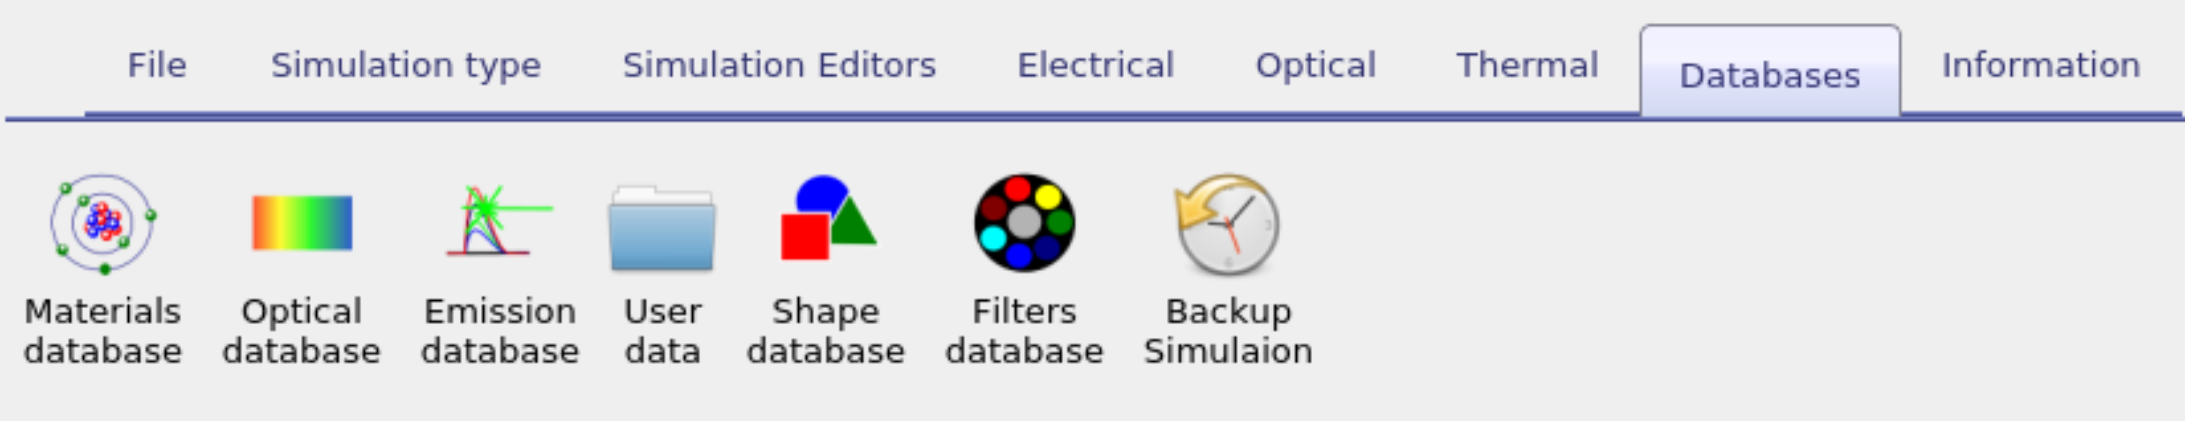
\includegraphics[width=0.7\textwidth]{./images/database_materials/database_ribbon.png}
\caption{The database ribbon}
\label{fig:database}
\end{figure}

There are two copies of these databases, one copy in the install directory of OghmaNano C:$\backslash$Program Files$\backslash$OghmaNano$\backslash$ and one in your home directory in a folder called oghma\_local.   When the model starts for the first time it copies the read only materials database from, to the oghma\_local folder in your home directory.  If you delete the copy of the materials database in the oghma\_local folder it will get copied back next time you start the model, this way you can always revert to the original databases if you damage the copy in oghma\_local.

The structure of the databases are simple, they are a series of directories with one directory dedicated to each material or spectra etc.. E.g. there will be one directory called Ag in the optical database which defines silver, and another directory in the spectra database called am1.5g which defines the solar spectrum.  Within each directory there is a data.json file which defines basic material properties of the material such as what it is and what icon to use for it.  There may be a couple of .bib files that contain reference information for the object in bibtex format. The rest of the key information will be stored in human readable .csv files. These files can be opend in notepad or any text editor. The one exception is that in the shape database some large files are stored in a binary format.
